\documentclass[border=12pt]{standalone}
\usepackage{tikz}
\usepackage{xcolor}
\usepackage{amsmath}
\usetikzlibrary{
  positioning,
  arrows.meta,
  fit,
  backgrounds,
  calc,
  shapes.geometric,
}

% ── Colour palette ──────────────────────────────────────────────────
\definecolor{textblue}{HTML}{4A90D9}
\definecolor{voicegreen}{HTML}{27AE60}
\definecolor{imagered}{HTML}{E74C3C}
\definecolor{recurrentpurple}{HTML}{8E44AD}
\definecolor{interleaveamber}{HTML}{F39C12}
\definecolor{darkgray}{HTML}{2C3E50}

% ── Styles ──────────────────────────────────────────────────────────
\tikzset{
  modbox/.style={
    draw=#1, fill=#1!8, rounded corners=4pt,
    minimum width=3.2cm, minimum height=0.8cm,
    font=\footnotesize\sffamily, align=center, line width=0.8pt,
  },
  widebox/.style={
    draw=#1, fill=#1!8, rounded corners=4pt,
    minimum height=0.8cm,
    font=\footnotesize\sffamily, align=center, line width=0.8pt,
  },
  annobox/.style={
    draw=#1!60, fill=#1!5, rounded corners=2pt,
    minimum width=2.4cm, minimum height=0.55cm,
    font=\scriptsize\sffamily, align=center, line width=0.5pt, dashed,
  },
  iolabel/.style={font=\scriptsize\sffamily\itshape, text=darkgray, align=center},
  attnlabel/.style={
    font=\tiny\sffamily\bfseries, rounded corners=2pt,
    fill=#1!15, draw=#1!40, inner sep=2pt,
  },
  groupbg/.style={
    draw=#1!40, fill=#1!4, rounded corners=6pt, line width=0.6pt, dashed,
  },
  arrow/.style={-{Stealth[length=5pt, width=4pt]}, line width=0.7pt, color=darkgray},
  thickarrow/.style={-{Stealth[length=6pt, width=5pt]}, line width=1.0pt, color=#1},
  dasharrow/.style={-{Stealth[length=5pt, width=4pt]}, line width=0.7pt, color=darkgray, dashed},
  thickdasharrow/.style={-{Stealth[length=6pt, width=5pt]}, line width=1.0pt, color=#1, dashed},
  seclabel/.style={font=\footnotesize\sffamily\bfseries, text=#1},
}

\begin{document}
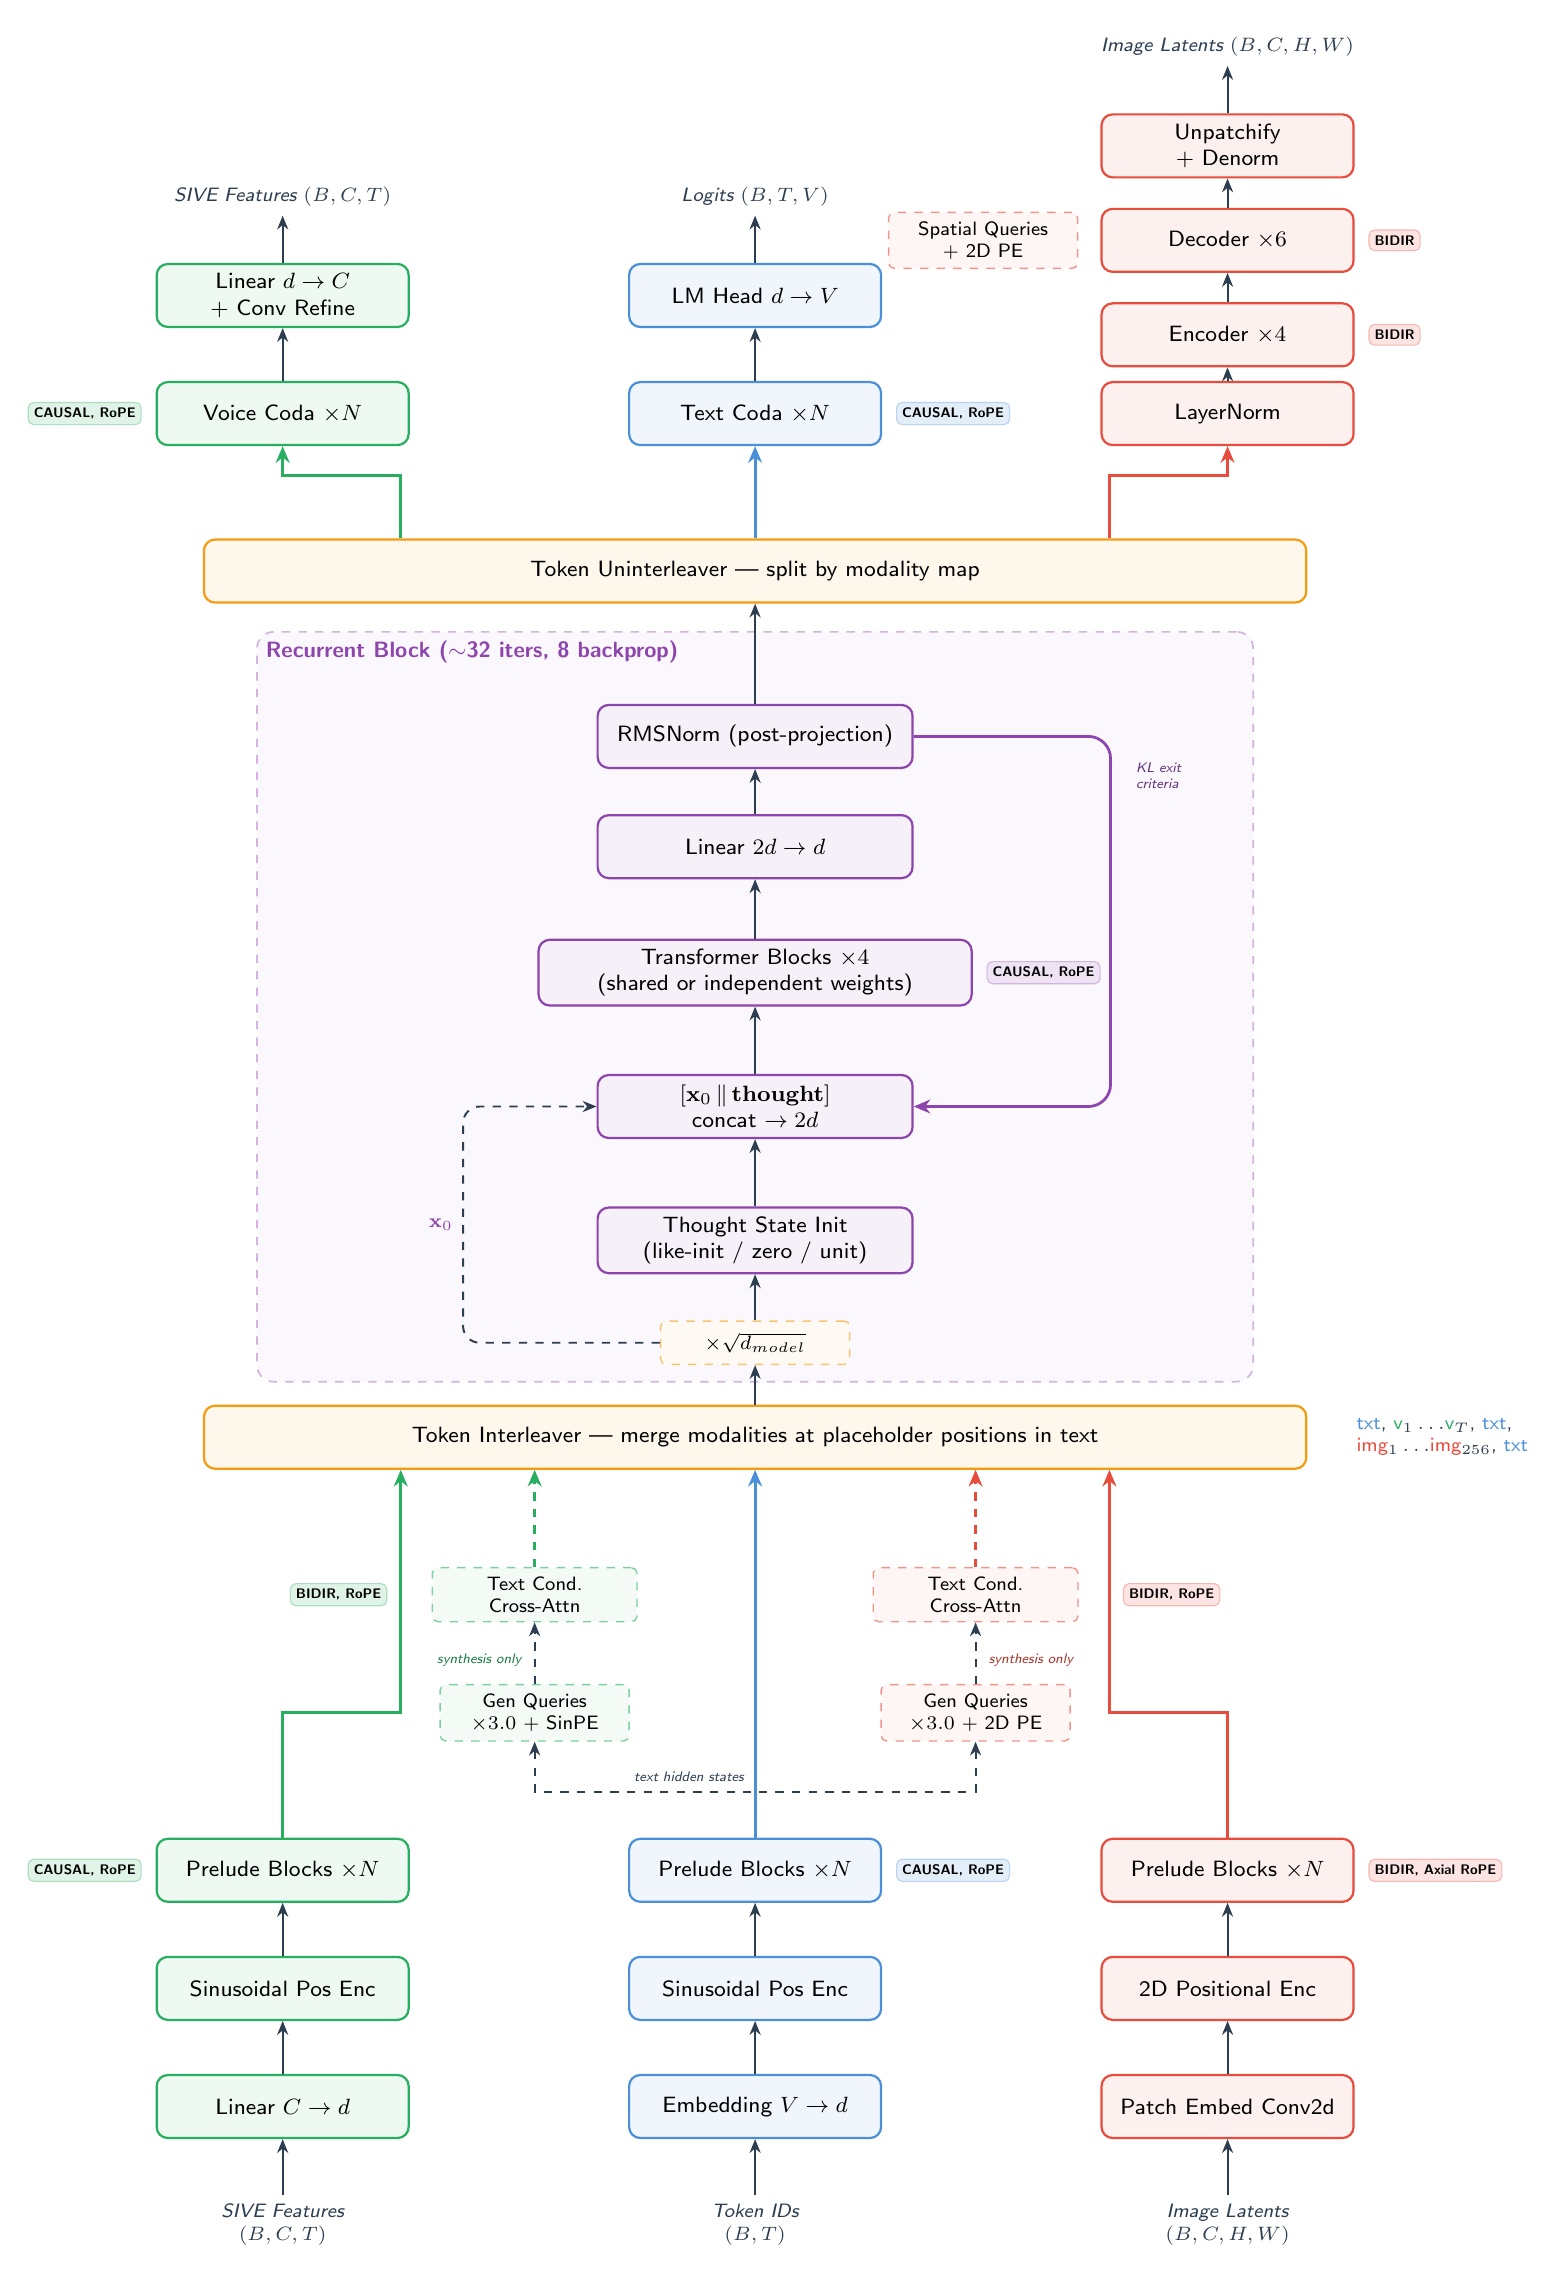
\begin{tikzpicture}

% Column X positions: voice - voiceCond - TEXT - imageCond - image
\def\voiceX{0}
\def\voiceCondX{3.2}
\def\textX{6}
\def\imageCondX{8.8}
\def\imageX{12}
\def\centerX{6}

% ════════════════════════════════════════════════════════════════════
% INPUTS (row 0)
% ════════════════════════════════════════════════════════════════════
\node[iolabel] (voice_in) at (\voiceX, 0) {SIVE Features\\$(B, C, T)$};
\node[iolabel] (text_in)  at (\textX, 0)  {Token IDs\\$(B, T)$};
\node[iolabel] (image_in) at (\imageX, 0) {Image Latents\\$(B, C, H, W)$};

% ════════════════════════════════════════════════════════════════════
% FEATURE EXTRACTORS / PRELUDES
% ════════════════════════════════════════════════════════════════════

% -- Voice (left) --
\node[modbox=voicegreen] (voice_proj)    at (\voiceX, 1.5) {Linear $C \to d$};
\node[modbox=voicegreen] (voice_pos)     at (\voiceX, 3.0) {Sinusoidal Pos Enc};
\node[modbox=voicegreen] (voice_prelude) at (\voiceX, 4.5) {Prelude Blocks $\times N$};
\node[attnlabel=voicegreen, anchor=east] at ([xshift=-5pt]voice_prelude.west) {CAUSAL, RoPE};

% -- Text (center) --
\node[modbox=textblue] (text_embed)   at (\textX, 1.5) {Embedding $V \to d$};
\node[modbox=textblue] (text_pos)     at (\textX, 3.0) {Sinusoidal Pos Enc};
\node[modbox=textblue] (text_prelude) at (\textX, 4.5) {Prelude Blocks $\times N$};
\node[attnlabel=textblue, anchor=west] at ([xshift=5pt]text_prelude.east) {CAUSAL, RoPE};

% -- Image (right) --
\node[modbox=imagered] (image_patch)   at (\imageX, 1.5) {Patch Embed Conv2d};
\node[modbox=imagered] (image_pos)     at (\imageX, 3.0) {2D Positional Enc};
\node[modbox=imagered] (image_prelude) at (\imageX, 4.5) {Prelude Blocks $\times N$};
\node[attnlabel=imagered, anchor=west] at ([xshift=5pt]image_prelude.east) {BIDIR, Axial RoPE};

% Prelude arrows
\draw[arrow] (voice_in) -- (voice_proj);
\draw[arrow] (voice_proj) -- (voice_pos);
\draw[arrow] (voice_pos) -- (voice_prelude);
\draw[arrow] (text_in) -- (text_embed);
\draw[arrow] (text_embed) -- (text_pos);
\draw[arrow] (text_pos) -- (text_prelude);
\draw[arrow] (image_in) -- (image_patch);
\draw[arrow] (image_patch) -- (image_pos);
\draw[arrow] (image_pos) -- (image_prelude);

% ════════════════════════════════════════════════════════════════════
% SYNTHESIS PATH: Gen Queries + Text Conditioning
% Text is in the center, so conditioning arrows fan outward cleanly.
% ════════════════════════════════════════════════════════════════════

% Voice synthesis (between voice and text)
\node[annobox=voicegreen] (voice_genq) at (\voiceCondX, 6.5) {Gen Queries\\$\times 3.0$ + SinPE};
\node[annobox=voicegreen, minimum width=2.6cm] (voice_textcond) at (\voiceCondX, 8.0) {Text Cond.\\Cross-Attn};
\node[attnlabel=voicegreen, anchor=east] at ([xshift=-16pt]voice_textcond.west) {BIDIR, RoPE};
\node[font=\tiny\sffamily\itshape, text=voicegreen!70!black, anchor=south]
  at ([xshift=-20pt,yshift=3pt]voice_genq.north) {synthesis only};

% Image synthesis (between text and image)
\node[annobox=imagered] (image_genq) at (\imageCondX, 6.5) {Gen Queries\\$\times 3.0$ + 2D PE};
\node[annobox=imagered, minimum width=2.6cm] (image_textcond) at (\imageCondX, 8.0) {Text Cond.\\Cross-Attn};
\node[attnlabel=imagered, anchor=west] at ([xshift=16pt]image_textcond.east) {BIDIR, RoPE};
\node[font=\tiny\sffamily\itshape, text=imagered!70!black, anchor=south]
  at ([xshift=20pt,yshift=3pt]image_genq.north) {synthesis only};

% Arrows for synthesis path
\draw[dasharrow] (voice_genq) -- (voice_textcond);
\draw[dasharrow] (image_genq) -- (image_textcond);

% Text feeds outward into both conditioning blocks (clean fan-out)
\draw[dasharrow] (text_prelude) -- ++(0, 1) -| (voice_genq)
  node[pos=0.15, above, font=\tiny\sffamily\itshape, text=darkgray] {text hidden states};
\draw[dasharrow] (text_prelude) -- ++(0, 1) -| (image_genq);

% ════════════════════════════════════════════════════════════════════
% TOKEN INTERLEAVER
% ════════════════════════════════════════════════════════════════════

\node[widebox=interleaveamber, minimum width=14cm] (interleaver) at (\centerX, 10.0)
  {Token Interleaver --- merge modalities at placeholder positions in text};

% Embed scale
\node[annobox=interleaveamber] (scale) at (\centerX, 11.2) {$\times \sqrt{d_{model}}$};

% Arrows into interleaver — from preludes and from text conditioning
\draw[thickarrow=voicegreen] (voice_prelude) -- ++(0, 2.0) -| ([xshift=-4.5cm]interleaver.south);
\draw[thickdasharrow=voicegreen] (voice_textcond) -- ++(0, 0.8) -| ([xshift=-2.8cm]interleaver.south);
\draw[thickarrow=textblue] (text_prelude) -- ++(0, 1.5) -| ([xshift=0cm]interleaver.south);
\draw[thickarrow=imagered] (image_prelude) -- ++(0, 2.0) -| ([xshift=4.5cm]interleaver.south);
\draw[thickdasharrow=imagered] (image_textcond) -- ++(0, 0.8) -| ([xshift=2.8cm]interleaver.south);

\draw[arrow] (interleaver) -- (scale);

% Interleaved sequence visualization
\node[font=\scriptsize\sffamily, text=darkgray, anchor=west, align=left]
  at ([xshift=0.5cm]interleaver.east)
  {{\color{textblue}txt}, {\color{voicegreen}v}$_1 \ldots${\color{voicegreen}v}$_T$,
   {\color{textblue}txt},\\
   {\color{imagered}img}$_1 \ldots${\color{imagered}img}$_{256}$,
   {\color{textblue}txt}};

% ════════════════════════════════════════════════════════════════════
% RECURRENT BLOCK
% ════════════════════════════════════════════════════════════════════

\node[modbox=recurrentpurple, minimum width=4.0cm] (thought_init) at (\centerX, 12.5)
  {Thought State Init\\(like-init / zero / unit)};

\node[modbox=recurrentpurple, minimum width=4.0cm] (combine) at (\centerX, 14.2)
  {$[\mathbf{x}_0 \,\|\, \mathbf{thought}]$\\concat $\to 2d$};

\node[modbox=recurrentpurple, minimum width=5.5cm] (recblocks) at (\centerX, 15.9)
  {Transformer Blocks $\times 4$\\(shared or independent weights)};
\node[attnlabel=recurrentpurple, anchor=west] at ([xshift=5pt]recblocks.east) {CAUSAL, RoPE};

\node[modbox=recurrentpurple, minimum width=4.0cm] (projection) at (\centerX, 17.5)
  {Linear $2d \to d$};

\node[modbox=recurrentpurple, minimum width=4.0cm] (postnorm) at (\centerX, 18.9)
  {RMSNorm (post-projection)};

% Background
\coordinate (rec_right_pad) at ([xshift=3.0cm]recblocks.east);
\coordinate (rec_left_pad) at ([xshift=-3.0cm]recblocks.west);
\begin{scope}[on background layer]
  \node[groupbg=recurrentpurple, inner sep=16pt,
    fit=(scale)(postnorm)(rec_right_pad)(rec_left_pad), yshift=10pt] (recbg) {};
\end{scope}

\node[seclabel=recurrentpurple, anchor=north west] at (recbg.north west)
  {Recurrent Block (${\sim}$32 iters, 8 backprop)};

% Arrows
\draw[arrow] (scale) -- (thought_init);
\draw[arrow] (thought_init) -- (combine);
\draw[arrow] (combine) -- (recblocks);
\draw[arrow] (recblocks) -- (projection);
\draw[arrow] (projection) -- (postnorm);

% Loop-back arrow — use node coordinates for precise alignment
\draw[thickarrow=recurrentpurple, rounded corners=8pt]
  (postnorm.east) -- ++(2.5, 0) |- (combine.east);

% x_0 injection (left side)
\draw[dasharrow, rounded corners=6pt]
  (scale.west) -- ++(-2.5, 0) |- (combine.west)
  node[pos=0.25, left, font=\scriptsize\sffamily\itshape, text=recurrentpurple] {$\mathbf{x}_0$};

% KL label on the loop-back arrow
\node[font=\tiny\sffamily\itshape, text=recurrentpurple!70!black, anchor=west, align=left]
  at ([xshift=2.7cm, yshift=-0.5cm]postnorm.east) {KL exit\\criteria};

% ════════════════════════════════════════════════════════════════════
% TOKEN UNINTERLEAVER
% ════════════════════════════════════════════════════════════════════

\node[widebox=interleaveamber, minimum width=14cm] (uninterleaver) at (\centerX, 21.0)
  {Token Uninterleaver --- split by modality map};

\draw[arrow] (postnorm) -- (uninterleaver);

% ════════════════════════════════════════════════════════════════════
% CODAS / GENERATORS
% ════════════════════════════════════════════════════════════════════

% Voice coda (left, matching input column)
\node[modbox=voicegreen] (voice_coda) at (\voiceX, 23.0) {Voice Coda $\times N$};
\node[modbox=voicegreen] (voice_proj_out) at (\voiceX, 24.5) {Linear $d \to C$\\+ Conv Refine};
\node[attnlabel=voicegreen, anchor=east] at ([xshift=-5pt]voice_coda.west) {CAUSAL, RoPE};

% Text coda (center, matching input column)
\node[modbox=textblue] (text_coda) at (\textX, 23.0) {Text Coda $\times N$};
\node[modbox=textblue] (text_lmhead) at (\textX, 24.5) {LM Head $d \to V$};
\node[attnlabel=textblue, anchor=west] at ([xshift=5pt]text_coda.east) {CAUSAL, RoPE};

% Image coda (right, matching input column — cross-attention architecture)
\node[modbox=imagered] (image_norm) at (\imageX, 23.0) {LayerNorm};
\node[modbox=imagered] (image_enc) at (\imageX, 24.0) {Encoder $\times 4$};
\node[attnlabel=imagered, anchor=west] at ([xshift=5pt]image_enc.east) {BIDIR};
\node[modbox=imagered] (image_dec) at (\imageX, 25.2) {Decoder $\times 6$};
\node[attnlabel=imagered, anchor=west] at ([xshift=5pt]image_dec.east) {BIDIR};
\node[modbox=imagered] (image_unpatch) at (\imageX, 26.4) {Unpatchify\\+ Denorm};

% Spatial queries feeding into decoder
\node[annobox=imagered, anchor=east] at ([xshift=-8pt]image_dec.west) {Spatial Queries\\+ 2D PE};

% Arrows from uninterleaver to codas
\draw[thickarrow=voicegreen] ([xshift=-4.5cm]uninterleaver.north) -- ++(0, 0.8) -| (voice_coda);
\draw[thickarrow=textblue]   ([xshift=0cm]uninterleaver.north) -- ++(0, 0.6) -| (text_coda);
\draw[thickarrow=imagered]   ([xshift=4.5cm]uninterleaver.north) -- ++(0, 0.8) -| (image_norm);

\draw[arrow] (voice_coda) -- (voice_proj_out);
\draw[arrow] (text_coda) -- (text_lmhead);
\draw[arrow] (image_norm) -- (image_enc);
\draw[arrow] (image_enc) -- (image_dec);
\draw[arrow] (image_dec) -- (image_unpatch);

% ════════════════════════════════════════════════════════════════════
% OUTPUTS
% ════════════════════════════════════════════════════════════════════

\node[iolabel, above=0.6cm of voice_proj_out] (voice_out) {SIVE Features $(B, C, T)$};
\node[iolabel, above=0.6cm of text_lmhead]    (text_out)  {Logits $(B, T, V)$};
\node[iolabel, above=0.6cm of image_unpatch]  (image_out) {Image Latents $(B, C, H, W)$};

\draw[arrow] (voice_proj_out) -- (voice_out);
\draw[arrow] (text_lmhead) -- (text_out);
\draw[arrow] (image_unpatch) -- (image_out);

\end{tikzpicture}
\end{document}
